\subsection{The interface}
\gls{igro} is a web platform fully developed in R with aid of Shiny libraries, combining the power of the R statistical instrument with HTML5/javascript flexibility.

Shiny apps are tipically designed for small applications, allowing a very easy and versatile way for developing and releasing them.
The basic structure of a shiny app is based on two main entities, the \gls{sui} and the \gls{ss}.
The first one includes all the aesthetic components which the user interact with, while the \gls{ss} processes all the computations.

Natively, shiny apps supports only one server, but when the needs grow up and multiple interfaces are needed the things become more complicated. 

Our case is composed of high number of methodologies for multiple-omics problem solving and required a more complex implementation.
To account our problematic, we choose to build \gls{igro} as self containing modules, by using recently born shiny modules technology \footnote{\url{https://shiny.rstudio.com/articles/modules.html}}.
In such a way, the main shiny app can be shredded in multiple "mini apps", each one with its own \gls{sui} and \gls{ss}.
This approach is totally invisible to the final user, but helps the developer for the maintainability and the extensibility of the entire tool.
Indeed, when future needs arise for the implementation of novel functionalities, it is necessary just to implement a novel module.

Our tool presents itself with an upper menu of main topics organized by main scopes. 
For each of these topics, a sub-menu with specific functionalities is available.
When additional functionalities are available, they appears in a left side menu.
In order to well setup the parameters for each functionality, an additional side menu is presented with the parameters and their possible values for the right setup (figure \ref{fig:integrhomain} shows a general representation of the main interface).

\begin{figure}[H]
\centering
\includegraphics[width=\textwidth, keepaspectratio]{img/integrho/interface.png}
\caption[\gls{igro} main interface]{\gls{igro} main interface description. A main menu in the upper part is presented with all the available main functionalities, and a left side menu is presented with additional functionalities (in blue). Red part indicates the settings for each functionality within the parameter setup. While in green results in table or graphical form are presented.}
\label{fig:integrhomain}
\end{figure}

Once the user set up the required parameters and used the section button the results are shown in graphical or table format in the main part of the interface.

Before to proceed to data analysis, it is mandatory for the user to setup the project with a dedicated interface. 
The user has to upload a design file which describes the information related to its samples, some of them are mandatory as the filename (with path) of the BAM files and the condition of each sample, while others are optional as the tissue or the run id. 
It is also possible to manually edit the design matrix directly from the interface (figure \ref{fig:integrhodesign}).

\begin{figure}[H]
\centering
\includegraphics[width=\textwidth, keepaspectratio]{img/integrho/design.png}
\caption[integrho design interface]{A screenshot of the project design \gls{igro} interface.}
\label{fig:integrhodesign}
\end{figure}

Using the project interface, \gls{igro} creates inside the working directory (returned by the \lstinline!getwd()! function) a dedicated folder with all the required subfolders and stores all the basic information of the project into an ad-hoc designed \lstinline!R6ProjectClass!, which is re-used during the whole session to speed up the configuration of each step of the analysis.


\subsection{Available Methodologies}

Unlike tools as Galaxy \cite{Hillman-Jackson2012} and Taverna \cite{Wolstencroft2013}, focused on analysis workflows, \gls{igro} gives to the user high freedom of interaction, reporting all performed steps in a human readable \textit{HTML} report.
 
It implements not only the methodologies reported inside \textit{ticorser} for \textit{RNA-Seq} and \textit{DEScan2} for \textit{ATAC-Seq}, but implements also methodologies for \textit{ChIP-Seq} data analysis, complementing these aspects by providing functionalities for their integration at different levels, such as functional enrichment with Gene Ontology and Pathways and peaks-genes annotation.

\begin{figure}[H]
\centering
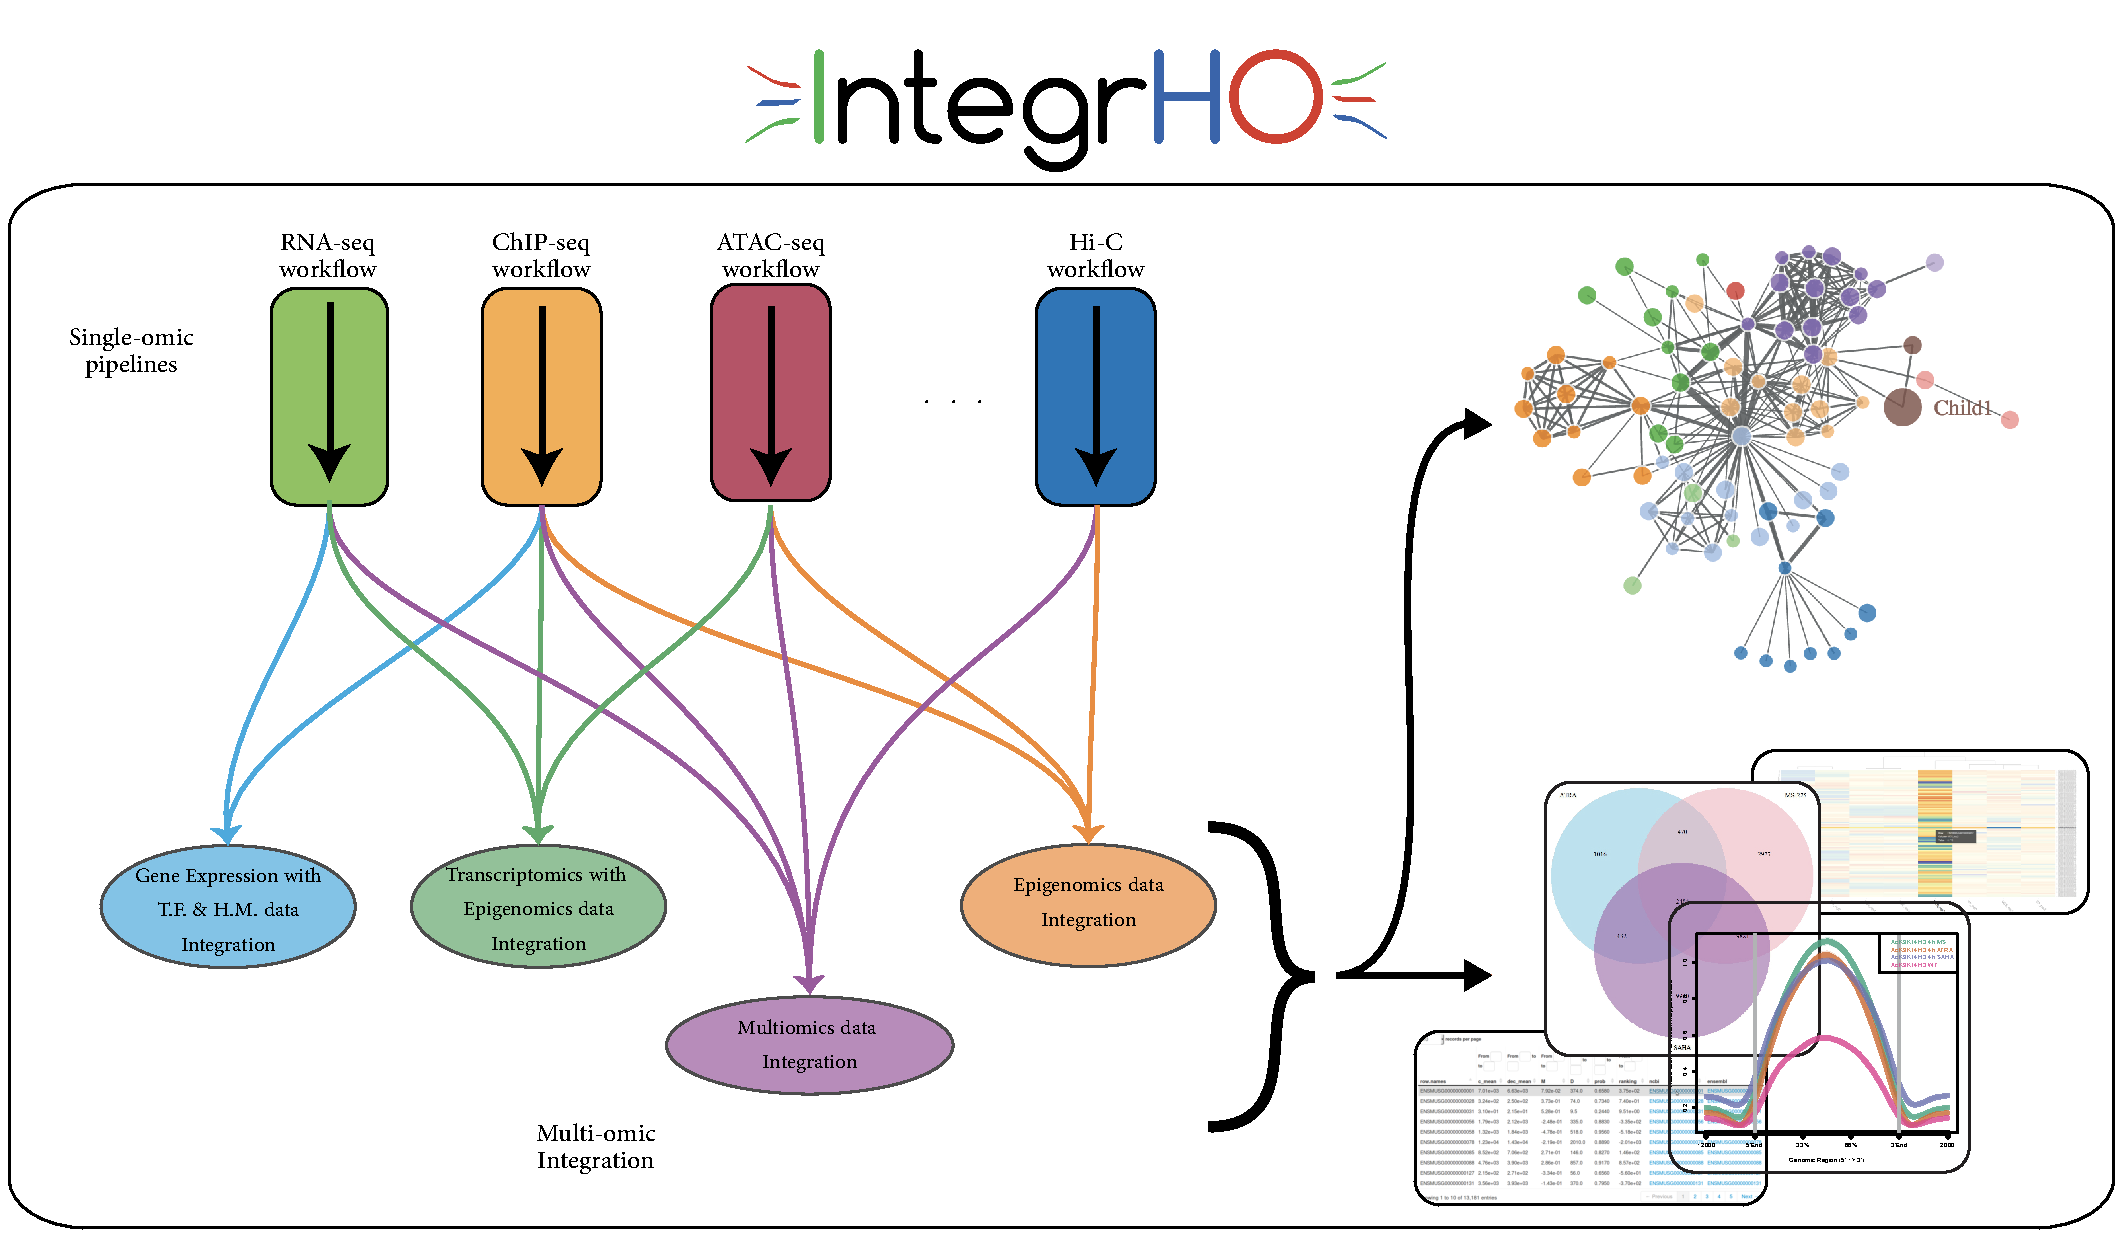
\includegraphics[width=\textwidth, keepaspectratio]{img/integrho/integrho_scheme.pdf}
\caption[integrho representation]{A schematical representation of \gls{igro} underlying idea.}
\label{fig:integrhoidea}
\end{figure}

For each -omics, \gls{igro} takes as input BAM or BED files, previously defined inside the design matrix of the main project definition interface.

Moreover, not only our software offers lots of utilities for data management and analysis, but also a great variability of graphics, useful to explore data and results, both in pre-processing and post-processing phase, such as \textit{barplots}, \textit{correlation plots}, \textit{heatmap}, \textit{scatterplots}, etc.

In order to facilitate the multi-omic data integration, we assembled several R functions to be freely combined in order to analyse each single-omic data type and to use their results for multi-omic data integration (Figure 1).

For \textit{RNA-seq} we constructed a dedicated interface for each step of a standard \textit{RNA-seq} data analysis pipeline, such as to build a count matrix, to filter out low counts with multiple tests, to normalize them and to account for batch effect.
Moreover, we selected multiple methods for \gls{deg}, such as \textit{edgeR}, \textit{DESeq2}, \textit{NOISeq}.

For \textit{ChIP-Seq} we constructed specific interfaces for peak calling, annotation and \glspl{der} detection.
For the peak calling, because of the lack of specific methods starting from BAM files, we implemented a dedicated interface for \textit{csaw}\cite{Lun2015} peak caller, which allows quantification for both broad and narrow peaks, typically resulting from \gls{hm} and \gls{tf} \textit{ChIP-seq} data.

For the annotation we selected the \textit{ChIPpeakAnno} and the \textit{ChIPseeker} R/Bioconductor packages, which produces similar output formats starting from peaks.
While for the detection of \glspl{der} we used the same methods as for \textit{RNA-seq}.

For \textit{ATAC-Seq} we used mostly the same methods implemented for the \textit{ChIP-Seq}, but designing specific interfaces for the filtering/alignment and the counting matrix as implemented in the \textit{DEScan2} package (see chapter \ref{sec:descan2cap} for further details).

To provide an integration of these -omics, we dedicated an entire section to this aspect, with functionalities for the annotation of \glspl{der} with \glspl{deg} using \textit{ChIPpeakAnno} and to use this information to investigate the functional response by enrichment for Gene Ontology or for Pathways.
These last two aspects implemented with aid of \textit{g:Profiler} \cite{Reimand2016} and \textit{graphite} \cite{Sales2012a} R/Bioconductor packages.
